\begin{tikzpicture}[
  font=\rmfamily,
  % Global styles
  node distance=1.2cm and 2.0cm,
  >=latex,
  box/.style={
    rectangle, rounded corners, thick, draw=black, align=center,
    minimum width=2.7cm, minimum height=1.0cm,
  },
  bigbox/.style={
    rectangle, dashed, draw=black!70, rounded corners,
    inner sep=0.4cm
  },
  arrowstyle/.style={->, thick},
  doublearrow/.style={<->, thick},
  titlebox/.style={font=\bfseries\Large},
]

\tikzset{
  computer fill/.initial=blue!20,
}

\tikzset{
  computer/.style n args={1}{%
    inner sep=0, % remove inner spacing so we have full control
    % Force a phantom so that the node gets a proper size.
    execute at begin node={\phantom{\rule{2.5cm}{1.75cm}}},
    draw=none, % don't draw the node's border
    % Everything is drawn in the path picture
    path picture={
      % Force the node's overall drawing area to include the base.
      \path[use as bounding box] (0,0) rectangle (2.5,1.75);
      % Draw the monitor rectangle.
      \draw[fill=\pgfkeysvalueof{/tikz/computer fill}] (0,0.25) rectangle (2.5,1.75);
      % Draw the two “leg” lines.
      \draw[fill=\pgfkeysvalueof{/tikz/computer fill}] (1.25,0.125) rectangle (1.5,.25);
      % Draw the base rectangle.
      \draw[fill=\pgfkeysvalueof{/tikz/computer fill}] (0.875,0) rectangle (1.875,0.125);
      % Place the text inside the monitor. (Here the monitor is 2cm wide and 1.5cm tall.)
      \node[anchor=center, align=center] at (0,1.5) {#1};
    }
  }
}

% ------------------------------------------------------------------------
% Two large dashed boxes for Particle Level (left) and Detector Level (right)
% ------------------------------------------------------------------------
\node[bigbox, label={[titlebox, xshift=0.cm, yshift=.75cm]\textcolor{black}{Reweighting Adversarial Networks}}](RANBox)
      at (4.875, 1) [minimum width=17.2cm, minimum height=10.2cm] {};

\node[bigbox, label={[titlebox, xshift=-1.cm, yshift=-1cm]
       \textcolor{green!40!black}{Particle Level}}] (particleBox)
      at (1,1) [minimum width=7.2cm, minimum height=8.2cm] {};

\node[bigbox, label={[titlebox, xshift=1cm, yshift=-1cm]
       \textcolor{blue!60!black}{Detector Level}}] (detectorBox)
      at (9,1) [minimum width=7.2cm, minimum height=8.2cm] {};

% ------------------------------------------------------------------------
% PARTICLE LEVEL NODES (within particleBox)
% ------------------------------------------------------------------------
% Generation (middle)
\node[computer={\textbf{Generation}\\[-1ex]\,}, computer fill=green!20]
    (gen) at ([xshift=3cm, yshift=-2.5cm] particleBox.north west){};

\node[align=center, opacity=0.75] (truth) [below=1.5cm of gen, xshift=2.5cm, inner sep=0pt, 
    label={[xshift=0.25cm,yshift=-0.5cm]center:{\shortstack{\textbf{Truth}}}}]{
    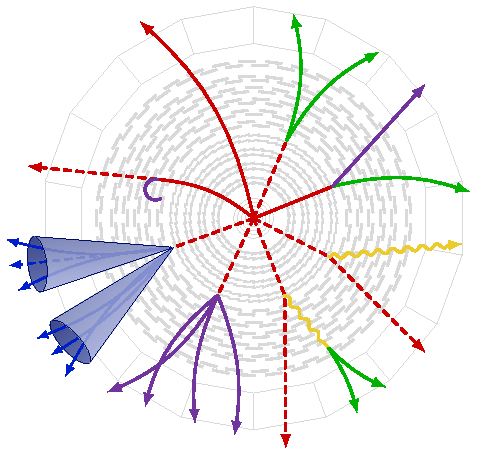
\includegraphics[width=0.25\linewidth]{figures/chapter-01/Collision.pdf}
};

% Re-weighted Generation (bottom)
\node[box, fill=green!10]
  (regen) [left=0.8cm of truth]
  {\textbf{Re-weighted}\\\textbf{Generation}};



% Arrow from Truth to Generation (optional, if needed conceptually)
\draw[draw=none] (regen) to node{\(\approx\)}(truth);

% Arrow from Generation to Re-weighted Generation
\draw[arrowstyle, red!70!black] (gen) -- node[midway, right, text=red!70!black, font=\bfseries] {\(\emph{g}\)} (regen);

% ------------------------------------------------------------------------
% DETECTOR LEVEL NODES (within detectorBox)
% ------------------------------------------------------------------------
% Data (top)
\node[computer={\textbf{Simulation}\\[-1ex]\;}]
  (sim) at ([xshift=3.5cm, yshift=-2.5cm]detectorBox.north west)
  {};

\node[align=center, opacity=0.75] (data) [below=0.9cm of sim, xshift=-1.5cm, inner sep=0pt, 
    label={center:{\shortstack{\textbf{Data}}}}]{
    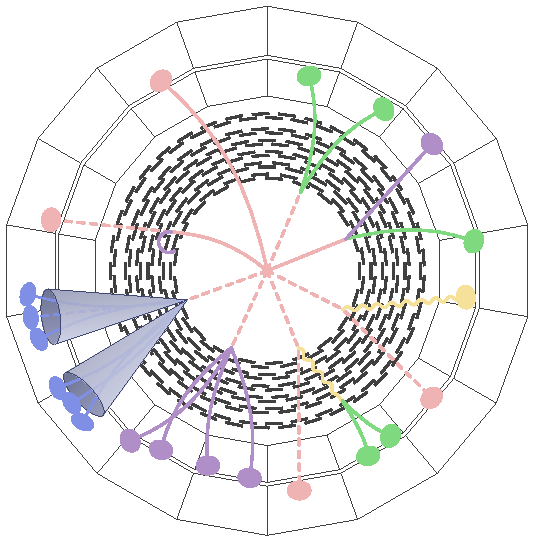
\includegraphics[width=0.25\linewidth]{figures/chapter-01/Collider.pdf}
};

% Re-weighted Simulation (bottom)
\node[box, fill=blue!10]
  (resim) [right=.5cm of data]
  {\textbf{Re-weighted}\\\textbf{Simulation}};



% ------------------------------------------------------------------------
% Connect the re-weighted generation to re-weighted simulation
% (Emulated detector arrow)
% ------------------------------------------------------------------------
\definecolor{Pink}{HTML}{FC9F5B}
\draw[arrowstyle,dashed,Pink, line width=1.2pt,
  decoration={
    markings,
    mark=at position 0.3 with {\node[above, rotate=22.5, font=\normalsize]{\textbf{Induced weights}};}
  },
  postaction={decorate}
]
  plot [smooth] coordinates {(regen.north east) (sim) ($(resim.north)+(0.2, 0)$)};

% ------------------------------------------------------------------------
% Double arrow between Data and Re-weighted Simulation (the discriminator)
% ------------------------------------------------------------------------
\path let \p1 = (data.north), \p2 = (resim.north) in
  node (dLabel) at ($(data)!0.5!(resim) + (0,2.0)$)
     {\textcolor{red!70!black}{$\mathbf{d}$}};

\draw[doublearrow, red!70!black]
  (data.north) to[out=90, in=270] (dLabel.south);
\draw[doublearrow, red!70!black]
  (dLabel.south) to[out=270, in=90] (resim.north);

% ------------------------------------------------------------------------
% Optional dashed arrow for backprop/update from discriminator to Re-weighted Generation
% ------------------------------------------------------------------------
\draw[arrowstyle, dashed, Pink, line width = 1.2pt]
  (dLabel) to[out=150, in=20] 
  node[pos=0.5, above, sloped, font=\normalsize]
    {\textbf{Backprop update}}
  ($(regen.east)+(-0.4,1.8)$);

\end{tikzpicture}